\subsection{Types}
Services calls usually return data in the JSON format. Javascript and Typescript are able to convert the JSON format into a class object.\\
Because of this, the \textit{EmporioLambda} Front-end module uses many not-primitive interfaces and classes in order to correctly convert the received JSON data. To send data, you can use the JSON.stringify function which converts an object passed as parameter into a JSON format string. The classes used can be found inside the src/objects folder.\\ Here's a class diagram that shows these classes and their dependencies between each other:
\vspace{0.5cm}
\begin{figure}[H]
\centering
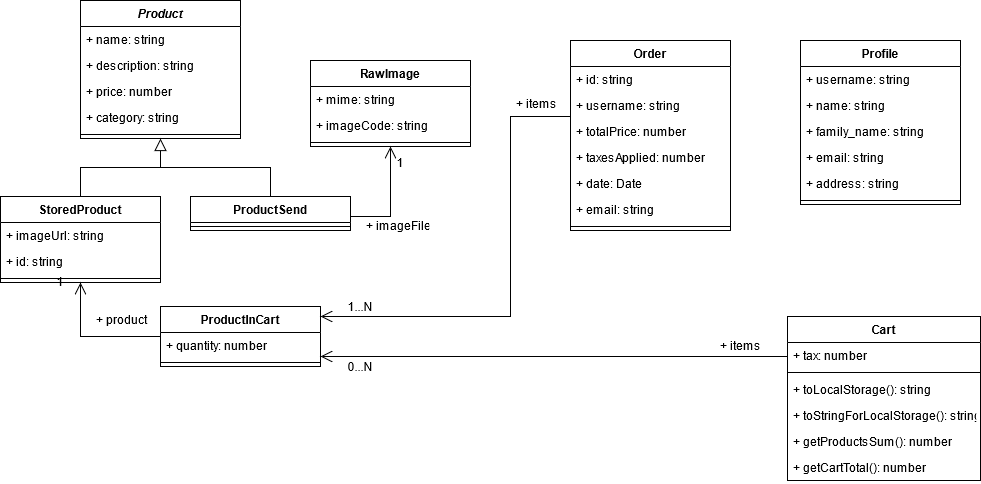
\includegraphics[scale=0.45]{res/Architettura/Frontend/img/class_frontend_types}\\
\caption{Diagram of the classes and types used in the Front-end module}
\end{figure}